\section{Object oriented project management}
\subsection{What is project management}
Project management is the use of specific knowledge, skills, tools and techniques to deliver something of value to people \cite{pmi}.

Project management is the discipline of initiating, planning, executing, controlling and closing the work of a team to achieve specific goals and meet specific success criteria. A project is temporary in that it has a defined beginning and end in time, and therefore defined scope and resources \cite{harelimana}.

\subsection{What is a project}
A project, on the other hand, is distinct in that it is not a routine action, but rather a specific group of operations aimed at achieving a single goal. As a result, a project team frequently consists of people who don't normally collaborate - perhaps from separate businesses and across several continents. Examples of projects can be the creation of software to improve a corporate process, the construction of a building or bridge, the relief effort following a natural disaster, expansion into a new geographical market.

\subsection{Object oriented project management}
\ac{o2pm} is based on concepts of Object oriented programming such as objects and attributes, classes and members. It consists of five major activities;

\begin{itemize}
\item finding classes and objects.
\item identifying structures.
\item identifying subjects.
\item defining attributes.
\item defining services.
\end{itemize}

Most importantly, \ac{o2pm} is all about applying the object-oriented approach to project management \cite{chandrashekar}.

Coming from the standpoint of \ac{o2pm}, every aspect of a project is an object. In a typical project setting, the project manager constructs a project plan using a tool, defines tasks, dates, and effort, and assigns them to team members; however there are possibly no adequate mechanisms to encapsulate work and define boundaries. This often will lead to accountability issues, challenges with effectively quantifying project milestones and producing inaccurate reports.

Many of these issues are addressed by \ac{o2pm}. The object-oriented approach to project management is the focus of O2PM, and the key characteristics are as follows:

\begin{itemize}
  \item \textbf{Encapsulation:} Team members can work well within defined bounds when work deliverables are encapsulated meaning that boundaries are well defined. Better control and, more crucially, accountability will result from this type of job encapsulation. It also aids in the easy identification of issues and their resolution.
  \item \textbf{Inheritance:} will specify the project's architecture, rules, standards, and processes, which must be “inherited” by all team members and their work deliverables.
  \item \textbf{Polymorphism:} Describes the concept that a singular object/interface can have several other implementations. For example, in a thesis project, the professor and student are different entities but both implement the same stakeholder class.
  \item \textbf{Communication:} This defines a known and standard medium through which each encapsulated work object communicates with each other.
\end{itemize}

\section{Object oriented programming}
\subsection{What is Object oriented programming}
\acl{oop} (\acs{oop}) is a programming paradigm that relies on the concept of classes and objects. It is used to structure a software program into simple, reusable pieces of code blueprints (called classes), which are used to create individual instances of objects. There are many object-oriented programming languages including JavaScript, C++, Java, and Python to name a few \cite{educative}.

\ac{oop} allows programmers to handle software development as if they were dealing with actual real-world objects. People, in everyday life, have the knowledge and ability to do a variety of duties. Objects in OOP have fields to hold knowledge, state, and data, as well as the ability to execute numerous methods.

A class in \ac{oop} serves as a blueprint for creating more specific objects. They represent broad categories that share attributes. They enforce what attributes their instances can have but the values for any specific instance is set by that instance itself. For example, in project management, a stakeholder is a party who has an interest in a specific activity and can either affect or be affected by the said activity. Now there are several types of stakeholders but in the OOP world, they are all different implementation of the parent class/blueprint, stakeholder. In order words, any specific type of stakeholder, will be represented as an object, which itself is a specific example of the rather generic class, stakeholder and will have unique values to the properties defined in the class.
\begin{figure}[h]
  \centering
  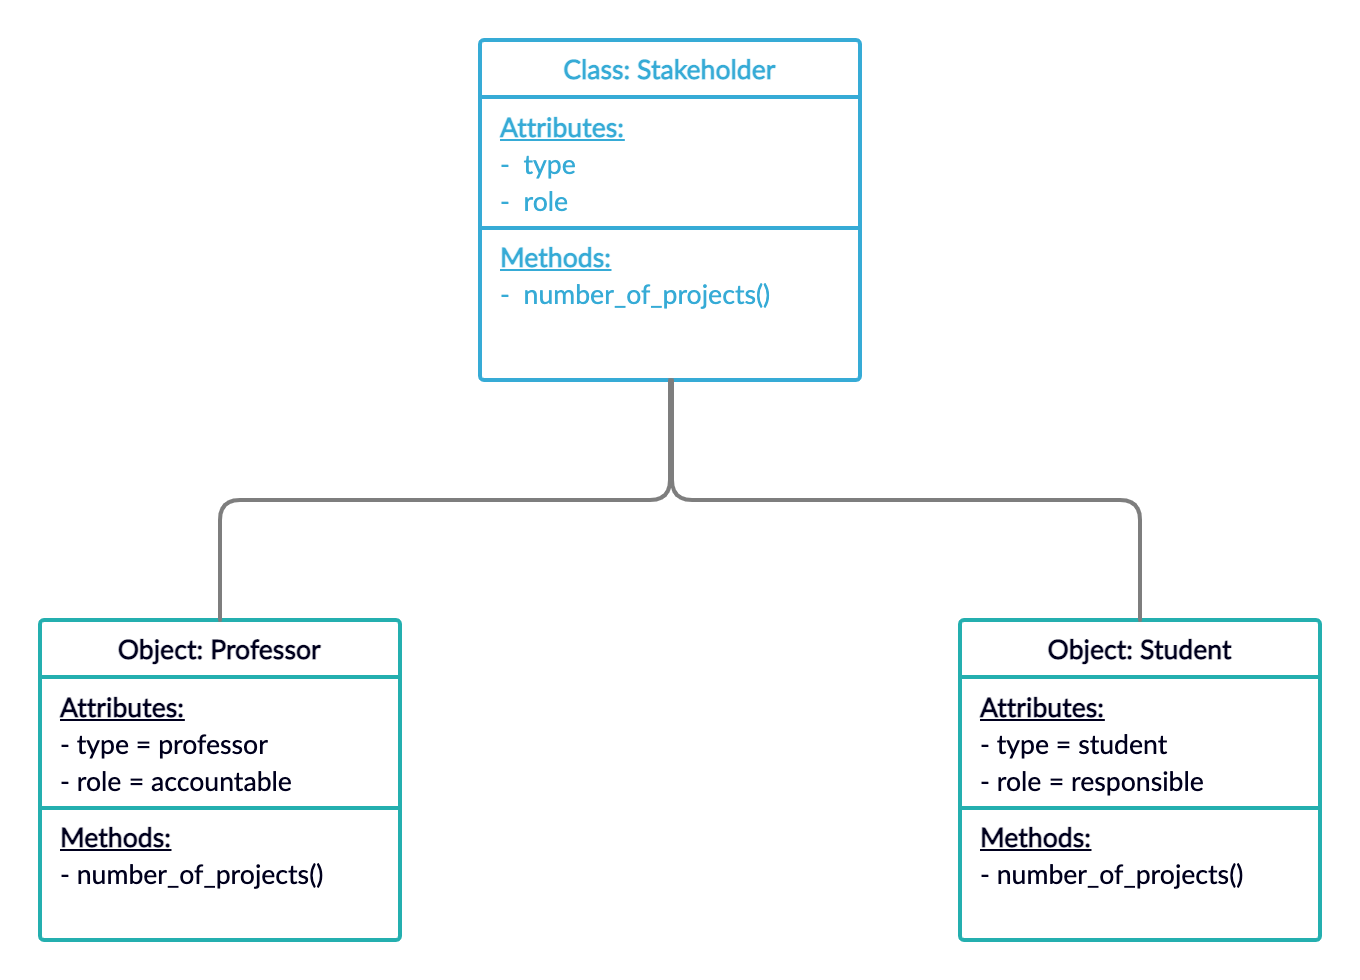
\includegraphics[width=130mm]{oop_illustration.png}
  \caption{Class Stakeholder implemented in Professor and Student class}
  \label{class blueprint}
\end{figure}

The above illustration visually depicts what has been explained so far. A Stakeholder class to contain all the properties a stakeholder must have and then from it are derived instances of a Stakeholder type object, Professor and Student to represent very specific stakeholders. Their attributes are isolated one from another and can be modified without affecting the original class or other objects. This means that the singular blueprint, Stakeholder can be reused to represent any number of stakeholders. The “role” field in the image above is according to RACI model which describes a responsibility assignment matrix.

The benefits that \acs{oop} presents are manyfold, from modelling complex things as simple reproducible structures to implementing objects that can be reused across programs to modifying the behavior of specific objects through polymorphism to their ability to protect information due to encapsulation.
It will be beneficial to explain some basic terminologies in OOP in the next section.

\subsection{Building blocks of OOP}
This section deals with elucidating the basic building blocks of an \acs{oop} program.

\subsubsection{Classes}
Classes are user-defined data types which is where the blueprint for the structure of attributes and methods are created. Individual objects can then be created or instantiated from this blueprint.

Classes have fields to hold attribute values and methods to model behavior. To illustrate, below is a code snippet in Python demonstrating how a generic class, \verb+Cat+ can be represented.
\begin{figure}[h]
  \centering
  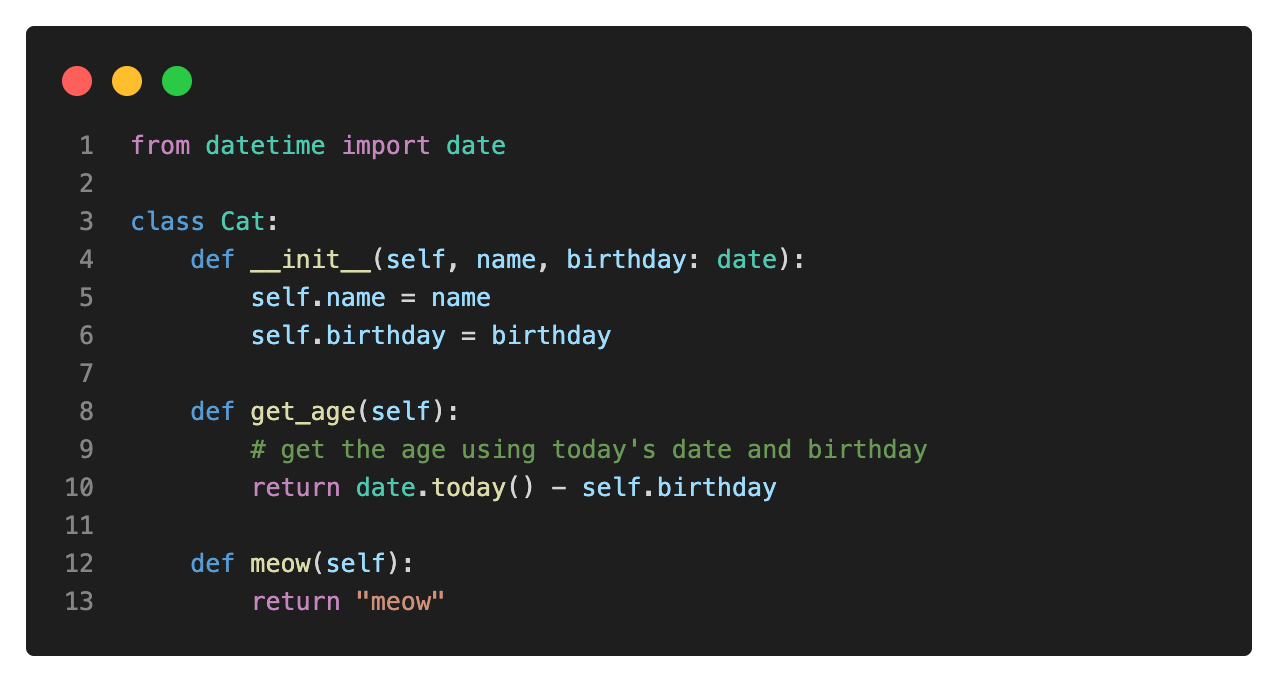
\includegraphics[width=130mm]{cat-code-snapshot.png}
  \caption{Cat class blueprint implementation}
  \label{cat class blueprint}
\end{figure}

The \verb+Cat+ class has attributes \verb+name+ and \verb+birthday+ and methods \verb+get_age()+ \verb+and meow()+.
With the knowledge that the class is only a blueprint for modelling a cat, a cat object can be instantiated from it to represent an individual real-world thing.

\subsubsection{Objects}
\ac{oop} is all about objects. Objects are instances of a class created with specific data. In code snippet, \verb+milana+ is an instance of the \verb+Cat+ class
\begin{figure}[h]
  \centering
  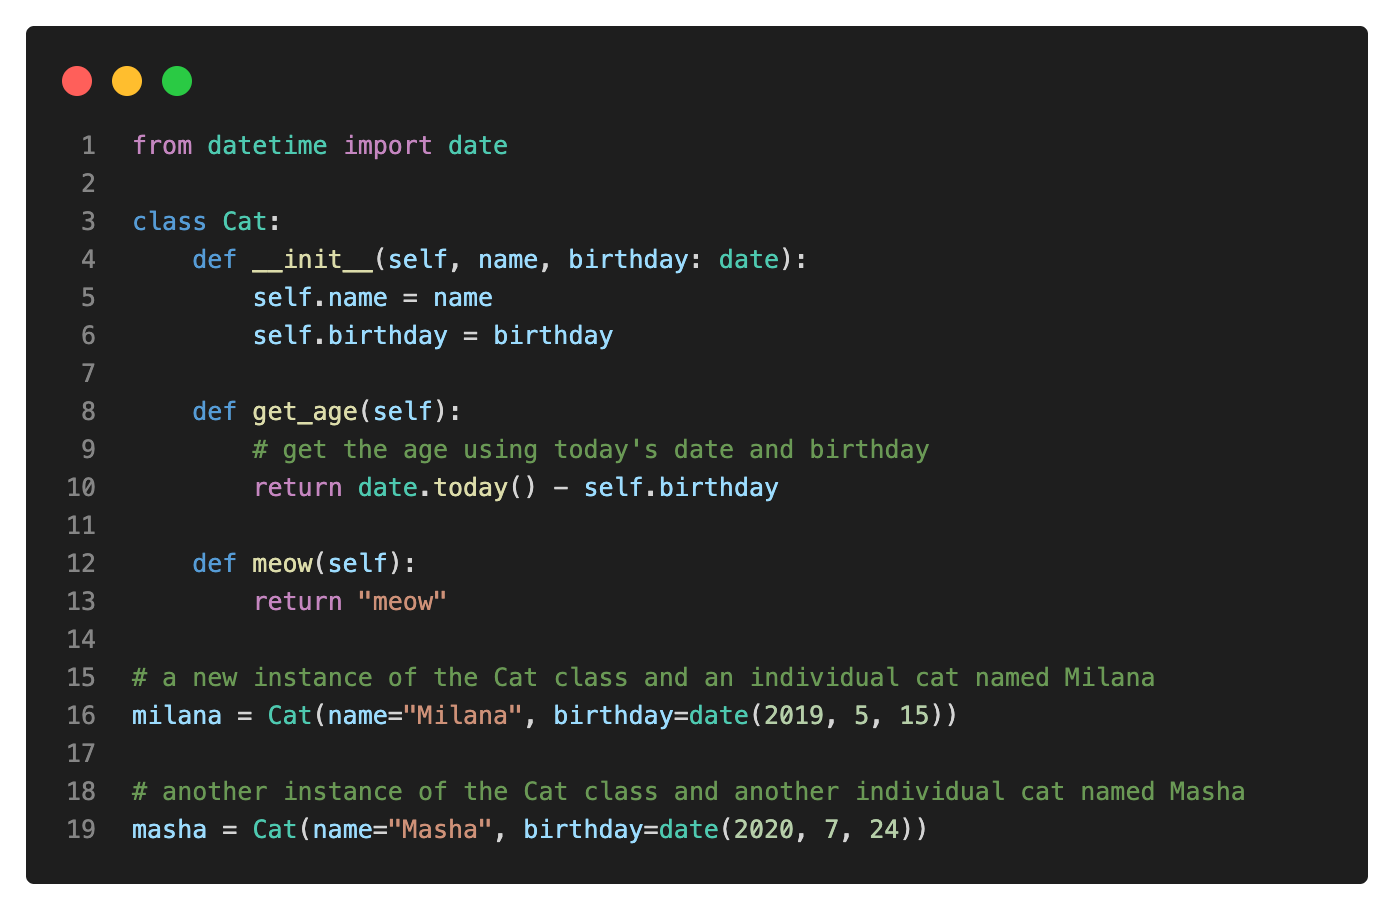
\includegraphics[width=130mm]{cat-instance-code-snapshot.png}
  \caption{Cat class instance}
  \label{cat class instance}
\end{figure}

When the \verb+Cat+ class is called like on lines 16 and 19:

\begin{itemize}
  \item A new object is created each time and stored in the variables \verb+milana+ and \verb+masha+ respectively.
  \item The constructor (\verb+__init__+) method runs with the \verb+name+ and \verb+birthday+ arguments and assigns values.
\end{itemize}

\subsubsection{Attributes}
The information that is stored is referred to as attributes. The Class template defines the attributes. Individual objects have data stored in the attributes field when they are instantiated.

The data in the object's attributes fields define the object's state. The \verb+birthday+ attribute could define the state of an object, allowing software to manage cats of various ages differently.

\subsubsection{Methods}
The behaviors of objects are represented by methods. Methods carry out operations, such as returning information about an object or updating its data. The code for the method is specified in the class definition.

Objects can invoke the methods described in the class when they are instantiated. In the code snippet below, the \verb+meow()+ method is defined in the \verb+Cat+ class and the \verb+meow()+ method is called on either the \verb+milana+ or \verb+masha+ object on lines 21 and 22 respectively.
\begin{figure}[h]
  \centering
  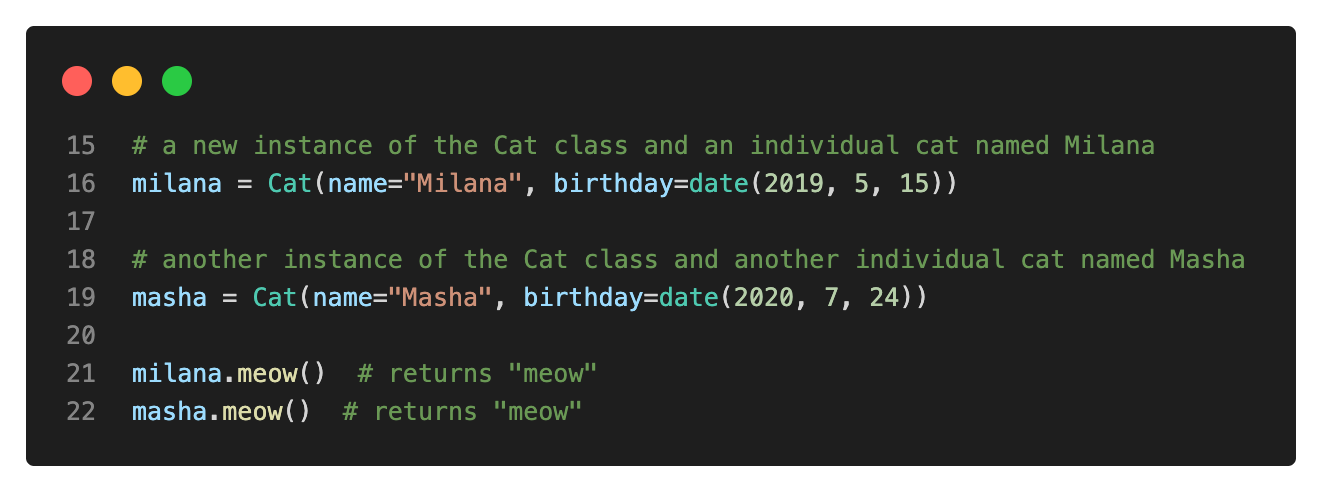
\includegraphics[width=130mm]{cat-instance-methods-code-snapshot.png}
  \caption{class methods}
  \label{cat class methods}
\end{figure}

Methods are often employed to modify, update or delete data but they don’t have to. As a matter of fact, the \verb+meow()+ method does not modify any data because meowing does not modify any of the attributes of the \verb+Cat+ class, \verb+name+ or \verb+birthday+.
Methods are how programmers keep functionality encapsulated within an object and promote reusability. When debugging, its reusability comes in handy. If an error occurs, there is only one location to look for it and correct it rather than numerous.

\section{Principles of \acs{oop}}
There are four main pillars of \acs{oop};
\begin{itemize}
  \item \textbf{Inheritance:} Child classes inherit data and behavior from their parent classes.
  \item \textbf{Encapsulation:} The process of enclosing information in an object and exposing only a necessary subset.
  \item \textbf{Abstraction:} exposing high-level public methods for accessing an object.
  \item \textbf{Polymorphism:} many methods can do the same task.
\end{itemize}

\subsubsection{Inheritance}
Objects typically have a lot in common. They have some similar logic. However, they are not comparable. Inheritance allows to reuse the common logic and extract the unique logic into another separate class. It implies that a (child) class can be created by deriving from another (parent) class. The child class derives all the parent class's fields and methods (common part) and can implement its own (unique part).

Herding dogs, for example, have a one-of-a-kind capacity to herd animals. To put it another way, all herding dogs are dogs, but not all dogs are herding dogs. This distinction can be illustrated by establishing a \verb+HerdingDog+ child class from a parent \verb+Dog+ class, and then adding the unique \verb+herd()+ behavior to it.

Inheritance has the advantage of allowing programs to build a generic parent class and then create more specific child classes as needed. This simplifies the overall development because, rather than duplicating the \verb+Dog+ class's structure repeatedly, child classes can have automatic access to their parent class's features.
\begin{figure}[H]
  \centering
  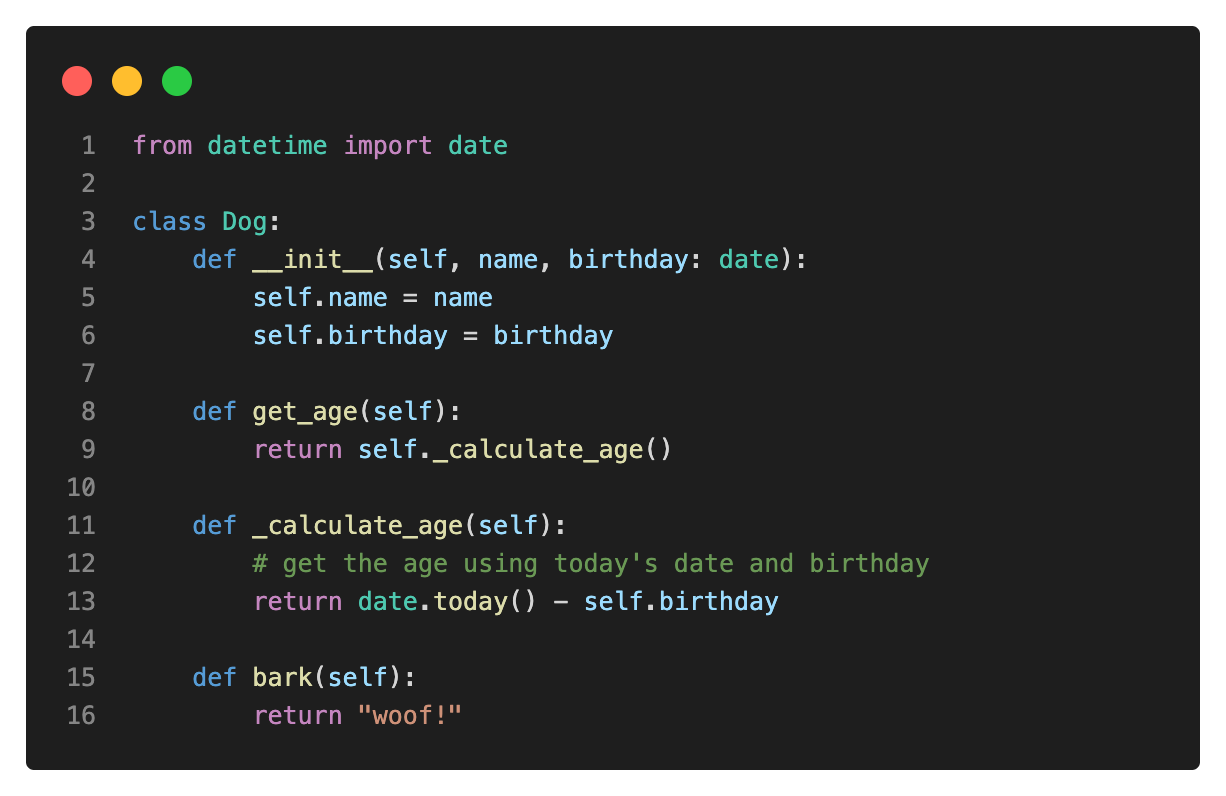
\includegraphics[width=130mm]{dog-code-snapshot.png}
  \caption{Generic Dog class}
  \label{generic dog class}
\end{figure}

In the code snippet in \autoref{inheritance illustration}, the child class \verb+HerdingDog+ inherits the method bark from the parent class \verb+Dog+ in \autoref{generic dog class} and adds a new method \verb+herd()+.
\begin{figure}[H]
  \centering
  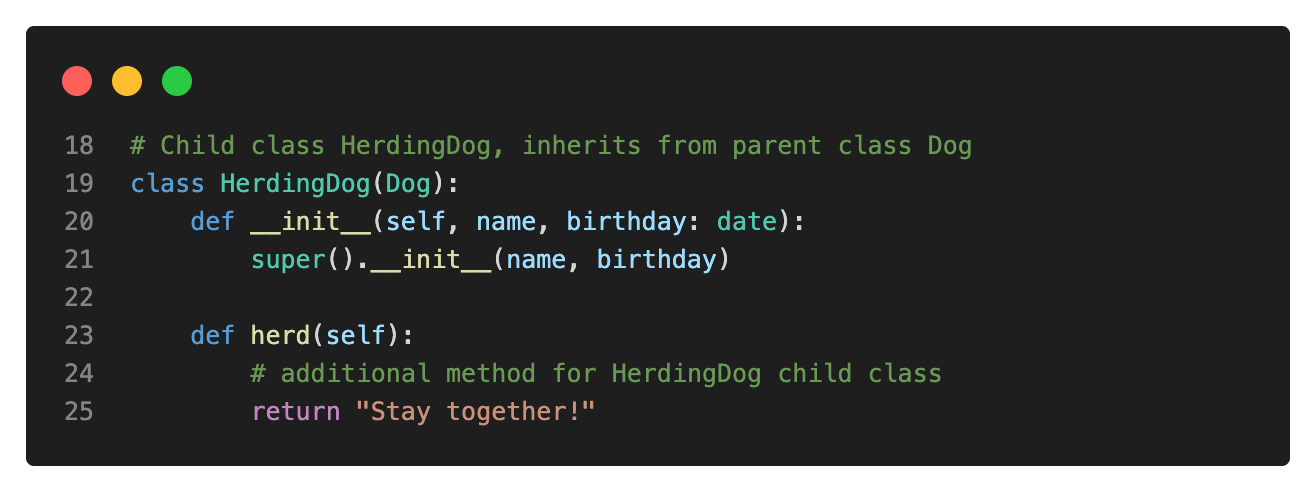
\includegraphics[width=130mm]{herd-dog-code-snapshot.png}
  \caption{Inheritance illustration}
  \label{inheritance illustration}
\end{figure}

The \verb+bark()+ method is not duplicated in the \verb+HerdingDog+ class; instead, it inherits the \verb+bark()+ method defined in the parent \verb+Dog+ class defined in \autoref{generic dog class}.

\begin{figure}[H]
  \centering
  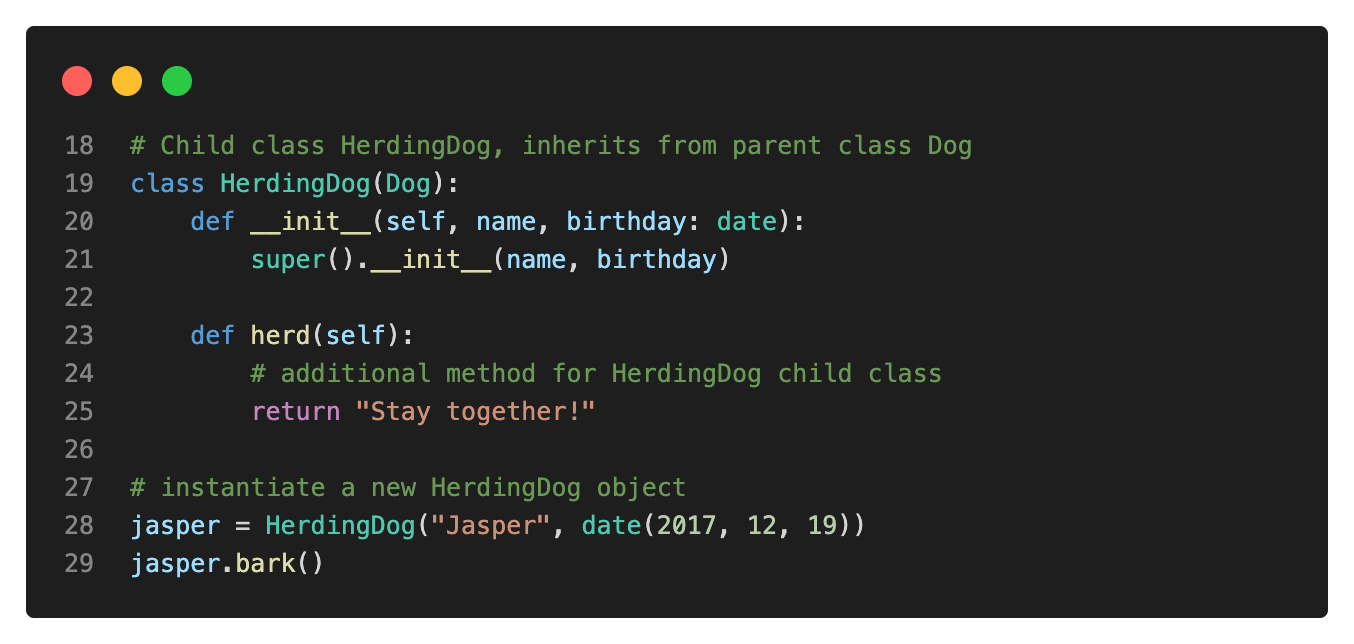
\includegraphics[width=130mm]{herd-dog-instance-code-snapshot.png}
  \caption{Child class instance}
  \label{child class instance}
\end{figure}

When the code in \autoref{cat class instance} calls \verb+jasper.bark()+ method, the \verb+bark()+ method traverses up the chain to the parent where the method has been defined.

\subsubsection{Encapsulation}
Encapsulation is the process of enclosing all critical information within an object and only presenting part of it to the outside world. Code within the class template defines attributes and behaviors.

Encapsulation hides the internal software code implementation inside a class and hides internal data of inside objects.

Encapsulation is achieved when each object keeps its state private, inside a class. Other objects don’t have direct access to this state. Instead, they can only call a list of public methods.

As an example of encapsulation, consider an automobile. Public interfaces are how the automobile communicates with the outside world by employing blinkers to signal turns. Under the hood, on the other hand, the engine is hidden.

Security is improved via encapsulation. Private attributes and methods can be defined to prevent access from outside the class. Public methods and properties are used to obtain or alter data in an object.

Using the \verb+Dog+ class example, encapsulation helps here so that access to private information on other \verb+Dog+ instances is not possible. Consider the \verb+get_age()+ method in \autoref{generic dog class}, the calculation is hidden inside the \verb+Dog+ class and each instance of the class will use the \verb+get_age()+ method to access the \verb+age+ data. Since methods can also update an object’s data, the developer controls what values can be changed through public methods.

\subsubsection{Abstraction}
Abstraction can be thought of as a natural extension of encapsulation. It refers to the user's interaction with only a subset of an object's attributes and operations. To access a complex object, abstraction use simplified, high-level tools. When employing abstraction, each object should only disclose a high-level mechanism for interacting with it. Internal implementation details should be hidden behind this mechanism. Using the automobile example again, you don’t have to know the details of the inner workings of the engine to drive it. The driver utilizes only a few tools, such as the gas pedal, brake, steering wheel, and blinker. The driver is not privy to the engineering. A lot of elements must function together under the hood to make an automobile run but revealing that knowledge to the driver would be a risky distraction.

In the \verb+Dog+ class example in \autoref{generic dog class}, the calculation of the age has been abstracted away into a private method \verb+_calculate_age()+ and a simple public method \verb+get_age()+ is exposed as a way to get the age information

The benefits of abstraction are summarized below:
\begin{itemize}
  \item Simple, high level user interfaces.
  \item Complex code is hidden.
  \item Security.
  \item Easier software maintenance.
  \item Updates to code will rarely change abstraction.
\end{itemize}

\subsubsection{Polymorphism}
Polymorphism refers to the design of items that have similar behavior. Objects can override shared parent behaviors with specific child behaviors through inheritance. Method overriding and method overloading are two ways that polymorphism allows the same method to perform various actions.

\begin{itemize}
  \item \textbf{Method Overriding} \\ In method overriding, the child class will provide its own implementation of a method already in the parent class effectively overriding it. If for the \verb+Dog+ class, there’s the need to create another child class \verb+TrackingDog+ which for some reason barks differently, the \verb+bark()+ method established in the parent class will have to be overridden like in the code snippet in \autoref{method overriding} to produce a different bark sound.

  \item \textbf{Method Overloading} \\ This kind of polymorphism happens at compile or code execution time. Methods may have the same name but behave differently based on the number of parameters passed to them.

  \begin{figure}[H]
    \centering
    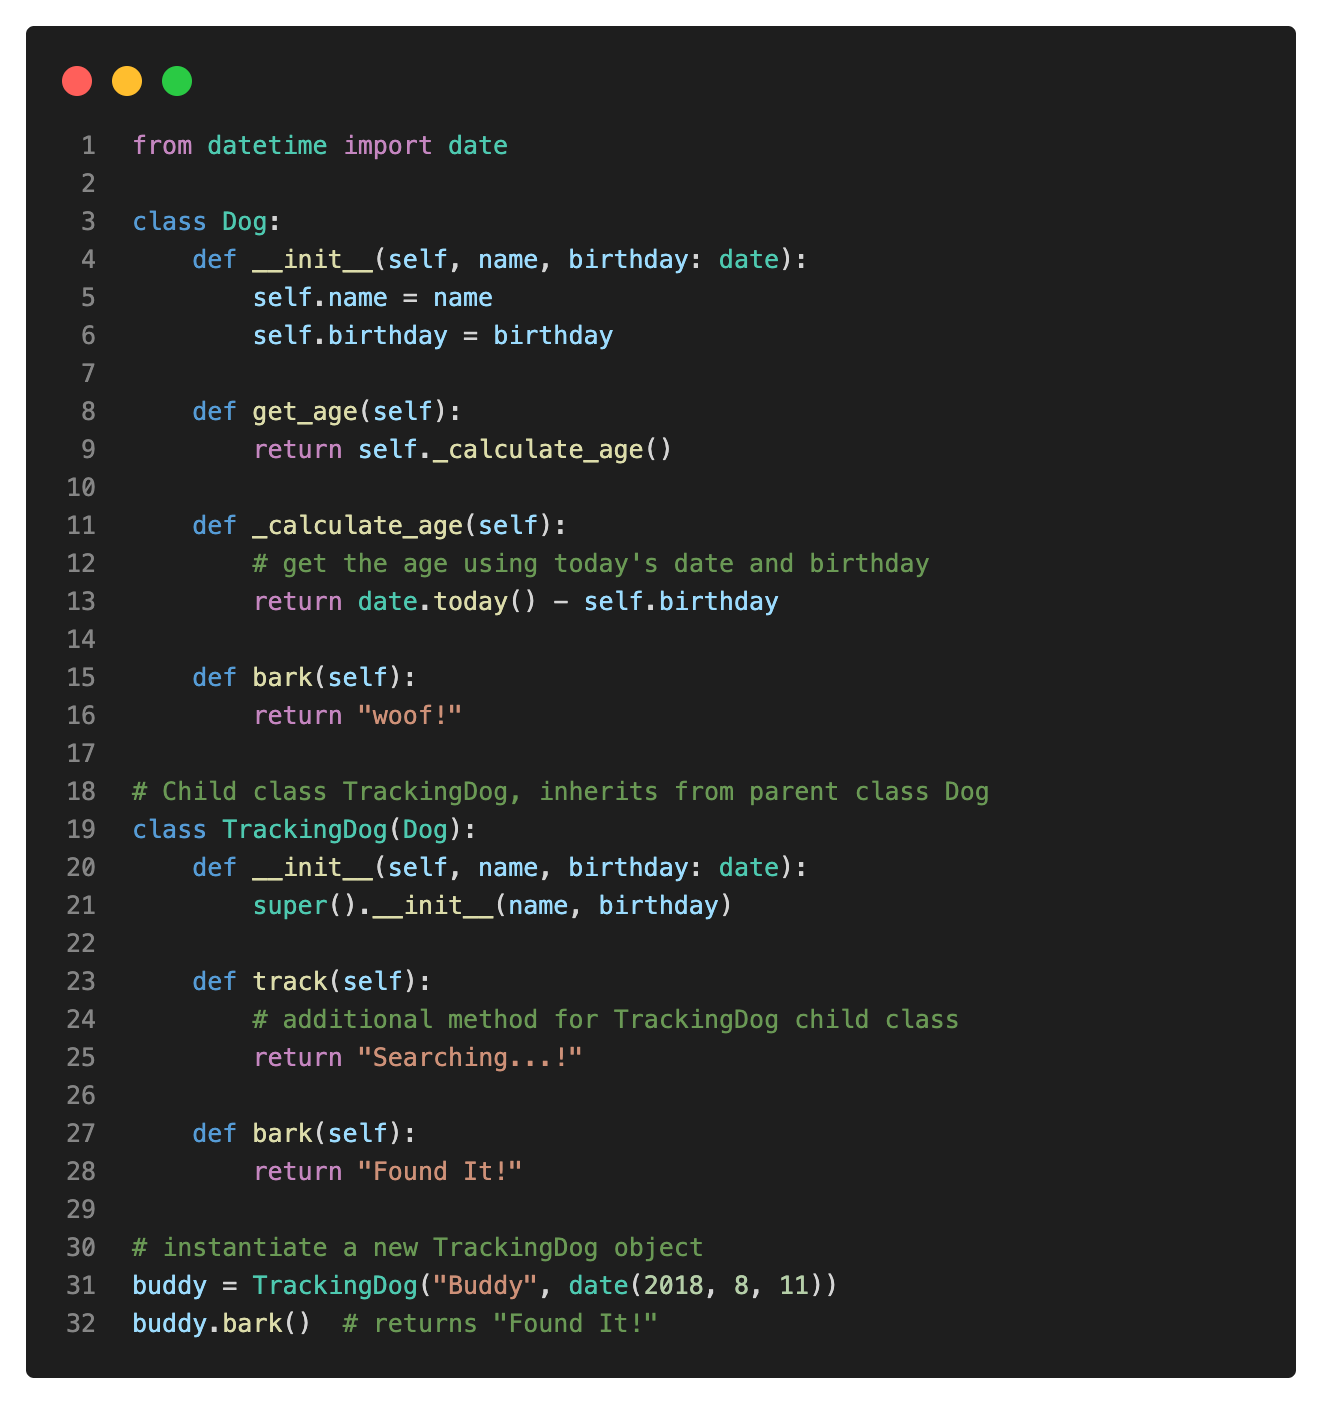
\includegraphics[width=130mm]{track-dog-overriding-instance-code-snapshot.png}
    \caption{Method overriding}
    \label{method overriding}
  \end{figure}
\end{itemize}

The benefits of Polymorphism are:

\begin{itemize}
  \item Objects of different types can be passed through the same interface.
  \item Method overriding.
  \item Method overloading.
\end{itemize}

\section{Libraries}
A "library" is a collection of program parts that do common and/or specialized things that save the programmer from needing to "reinvent the wheel" when writing software. A class library is a pre-coded OOP template collection. It usually consists of functions to call and object classes you can instantiate \cite{stevenparker}.

Libraries encourage code reuse and decrease redundancy by providing implementation of repetitive jobs.  Developing programs from the ground up can be a time-consuming and costly task. Class libraries include all necessary classes in a previously written coded format, making programming easier while also improving code quality. Customizing the class template is done in accordance with the programming requirements. To minimize programming language limitations, class libraries are regularly updated, and time verified for stability.

Programmers can decide to build everything from the ground up, but this is incredibly unsustainable and ill-advised for the reasons below;

\begin{itemize}
  \item \textbf{Expertise in the domain covered by the library:} Authors are usually experts in the domain covered by the library. This will ensure that users of the library get the best implementation possible.
  \item \textbf{Stability:} Libraries have the benefit of being used by hundreds, if not thousands, of developers around the world. Most of the early issues have already been encountered and resolved by authors.
  \item \textbf{Knowledge:} By having to use code pre-written by others, developers gain knowledge in the process. Many well-known libraries are built by top developers and serve as excellent examples of solid coding and design.
  \item \textbf{Finances:} For commercial libraries, the equivalent of hundreds, if not thousands, of man days of work can be got for free thanks to open source.
\end{itemize}

\section{Overview of the thesis}
To be done